\section{Visual Object Models}
\label{sec:visual-object-models}

An object model is a computational answer to a deceptively simple question: what
does an object look like, expressed in a form an algorithm can search for? A
person has no trouble saying that a coffee mug has a rounded body and a handle,
but a detector needs something concrete: a parametric shape, a set of edge
displacements, a collection of characteristic image patches, or a learned
feature map. The shape of that representation decides which transformations the
detector can tolerate (translation, scale, rotation, partial occlusion) and how
the search through the image is organized.

This section develops object models through a single recurring idea that ties
its parts together:

\begin{quote}
\emph{Local image evidence accumulates into global object hypotheses by voting.}
\end{quote}

\noindent
Each fragment of the image (an edge, a gradient, a patch) is weak and ambiguous
on its own, but it is consistent with only a limited set of global explanations.
If every fragment casts a vote for the explanations it supports, the correct
hypothesis collects many votes and stands out as a peak in a parameter space,
while accidental coincidences stay near the noise floor. We follow this idea
through increasingly flexible models: edges first vote for \emph{lines}
(Hough transform), then for the center of a \emph{known shape} (generalized
Hough transform), and finally learned appearance \emph{parts} vote for the
center of an \emph{object category} (implicit shape model). Saliency and
descriptors sit in between, deciding \emph{which} local evidence is worth
trusting in the first place.

\subsection{Detecting Lines: The Hough Transform}

The simplest non-trivial object model is a straight line, possibly broken by
noise or occlusion into many short edge fragments. The difficulty is that the
fragments are scattered across the image, and we do not know in advance how many
lines there are or where they lie. Testing every possible line against every
group of pixels would be hopeless. The Hough transform sidesteps this by changing
coordinates: instead of grouping pixels in the image, it lets every pixel vote in
the space of all possible \emph{lines}, and then simply looks for the lines that
received many votes.

To make ``the space of all lines'' concrete we need a way to label each line by a
few numbers. The familiar slope--intercept form $y = mx + b$ is a poor choice: a
vertical line has infinite slope, so $m$ and $b$ cannot represent it. The
\emph{Hesse normal form} sidesteps this by describing a line through the one point
it can never help but single out --- the point on the line closest to the origin.

Every line has a unique closest point to the origin: the foot of the perpendicular
dropped from the origin onto the line. We can reach that foot by starting at the
origin and walking a fixed distance $r \ge 0$ in a single direction. Call $\theta$
the angle of that direction, so the unit vector pointing from the origin straight
at the line is
\begin{equation}
  \hat{\mathbf n} = (\cos\theta,\ \sin\theta),
  \label{eq:unit-normal}
\end{equation}
\noindent
so the foot of the perpendicular is the point
\begin{equation}
  P_0 = r\,\hat{\mathbf n} = (r\cos\theta,\ r\sin\theta).
  \label{eq:foot}
\end{equation}
\noindent
The vector from the origin to $P_0$ is $r$ times $\hat{\mathbf n}$, so it is
\emph{normal} (perpendicular) to the line, because the shortest path from a point
to a line always meets it at a right angle. The pair $(r,\theta)$ then pins the
line down completely: $\theta$ says which way the line faces and $r$ says how far
out it lies.

To turn this picture into an equation, take any point $P = (x,y)$ on the line and
look at the vector $P - P_0$ that runs from the foot to it. Because both $P$ and
$P_0$ lie on the line, this vector points \emph{along} the line; and the line is
perpendicular to the origin-to-foot vector $P_0$. Orthogonality of $P - P_0$ and
$P_0$ means their dot product vanishes,
\begin{equation}
  (P - P_0)\cdot P_0 = 0
  \qquad\Longleftrightarrow\qquad
  P\cdot P_0 = P_0\cdot P_0 .
  \label{eq:ortho}
\end{equation}
\noindent
Both sides are now immediate. On the left,
$P\cdot P_0 = x\,(r\cos\theta) + y\,(r\sin\theta) = r\,(x\cos\theta + y\sin\theta)$;
on the right,
$P_0\cdot P_0 = r^2(\cos^2\theta + \sin^2\theta) = r^2$, using
$\cos^2\theta + \sin^2\theta = 1$. Equating the two gives
$r\,(x\cos\theta + y\sin\theta) = r^2$, and cancelling one factor of $r$ (every
line we care about has $r > 0$) leaves the Hesse normal form of the line,
\begin{equation}
  x\cos\theta + y\sin\theta = r .
  \label{eq:line-rtheta}
\end{equation}
\noindent
Figure~\ref{fig:hesse} shows the whole construction. What looked like an arbitrary
combination of a cosine and a sine is really one clean geometric statement: from
every point $P$ on the line, the step $P - P_0$ to the foot leaves at a right angle
to the origin-to-foot vector $P_0$.

\begin{figure}[ht]
  \centering
  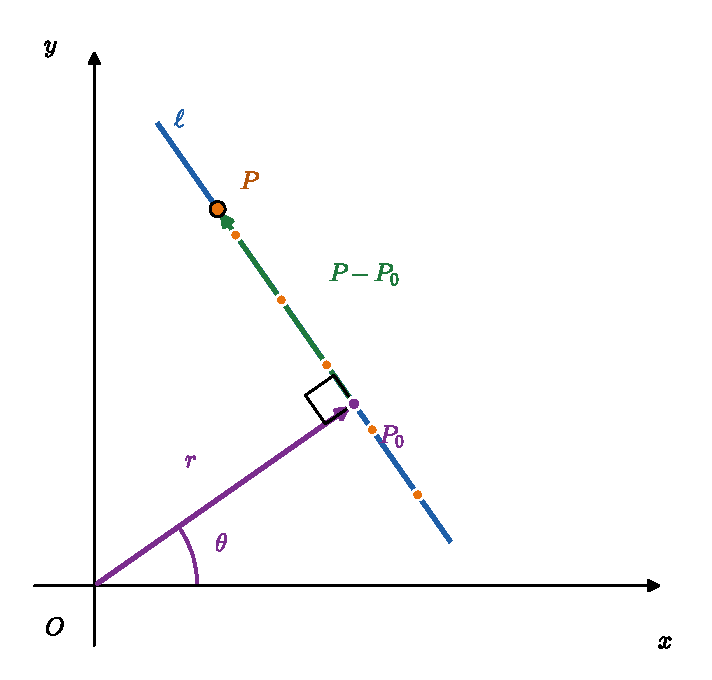
\includegraphics[width=0.52\textwidth]{figures/hesse_normal_form.pdf}
  \caption{The Hesse normal form of a line. The foot of the perpendicular from the
  origin $O$ is $P_0 = (r\cos\theta,\,r\sin\theta)$, reached by walking a distance
  $r$ at angle $\theta$. For any point $P$ on the line $\ell$, the vector $P - P_0$
  runs along the line and is therefore orthogonal to $P_0$; the condition
  $(P-P_0)\cdot P_0 = 0$ is exactly $x\cos\theta + y\sin\theta = r$, which every
  collinear edge point (orange) satisfies with the same $(r,\theta)$.}
  \label{fig:hesse}
\end{figure}

\noindent
Here $x$ and $y$ are pixel coordinates, $r \ge 0$ is measured in pixels, and
$\theta$ ranges over $[0,\pi)$. A quick sanity check fixes the meaning of the two
numbers. A horizontal line at height $y = c$ has a vertical perpendicular, so
$\theta = 90^\circ$ and Equation~\eqref{eq:line-rtheta} reduces to $r = c$; a
vertical line $x = d$ has $\theta = 0^\circ$ and $r = d$; a line passing through
the origin has $r = 0$ at every one of its points, whatever its angle. No line,
not even a vertical one, makes the parameters blow up. That is exactly the
robustness the slope--intercept form lacks.

The decisive property of Equation~\eqref{eq:line-rtheta} is an \emph{invariance}:
every pixel that lies on one particular line produces the \emph{same} pair
$(r,\theta)$, because $r$ and $\theta$ describe the line, not the individual
point. A whole line in the image therefore collapses to a single point in the
$(r,\theta)$ \emph{parameter space}. Now read the same equation the other way
around. Fix a single image point $(x_0,y_0)$ and let $\theta$ vary; the equation
turns into a function of $\theta$ alone,
\begin{equation}
  r(\theta) = x_0\cos\theta + y_0\sin\theta ,
  \label{eq:point-r-of-theta}
\end{equation}
\noindent
a fixed weighted sum of a cosine and a sine. Any such combination collapses to a
single shifted sine of the same frequency, and it is worth seeing exactly why,
because the shift is where the phase $\varphi$ comes from. Write down the shifted
sine we are aiming for and expand it with the angle-addition identity
$\sin(\alpha+\beta) = \sin\alpha\cos\beta + \cos\alpha\sin\beta$:
\begin{equation}
  R\,\sin(\theta + \varphi)
    = \underbrace{R\cos\varphi}_{\text{weight of }\sin\theta}\,\sin\theta
    + \underbrace{R\sin\varphi}_{\text{weight of }\cos\theta}\,\cos\theta .
  \label{eq:phase-expand}
\end{equation}
\noindent
For this to equal $x_0\cos\theta + y_0\sin\theta$ for \emph{every} $\theta$, the
two expressions must have the same weight on $\cos\theta$ and the same weight on
$\sin\theta$ separately. Matching them term by term gives
\begin{equation}
  x_0 = R\sin\varphi, \qquad y_0 = R\cos\varphi .
  \label{eq:phase-match}
\end{equation}
\noindent
These two relations determine $R$ and $\varphi$ from the point alone. Squaring and
adding them cancels $\varphi$ (via $\sin^2+\cos^2 = 1$) and leaves the amplitude,
\begin{equation}
  R = \sqrt{x_0^2 + y_0^2},
  \label{eq:phase-amp}
\end{equation}
\noindent
which is simply the point's distance from the origin; dividing them instead cancels
$R$ and fixes the phase,
\begin{equation}
  \varphi = \operatorname{atan2}(x_0,\, y_0).
  \label{eq:phase-phi}
\end{equation}
\noindent
Here $\operatorname{atan2}$ is the two-argument arctangent, which recovers the
angle in the correct quadrant from the signed pair $(x_0,y_0)$. So $\varphi$ is not
a new free parameter that appears from nowhere: it is the phase
\emph{forced} on the sinusoid by where the point sits, namely the angle of
$(x_0,y_0)$ measured from the $y$-axis (that is what
Equation~\eqref{eq:phase-match} says, since $(x_0,y_0)=(R\sin\varphi,R\cos\varphi)$).
Reassembling the pieces,
\begin{equation}
  r(\theta) = x_0\cos\theta + y_0\sin\theta = R\,\sin(\theta + \varphi),
  \label{eq:point-sinusoid}
\end{equation}
\noindent
which is a sinusoid in the $(r,\theta)$ plane whose amplitude $R$ is just the
point's distance from the origin and whose phase $\varphi$ encodes its direction.
The sinusoid enumerates \emph{all} the lines
that pass through that one point. Two pixels that happen to lie on a common line
have sinusoids that cross at the $(r,\theta)$ of that shared line; many collinear
pixels produce many sinusoids crossing at a single point. That crossing is the
peak we are looking for. Figure~\ref{fig:hough-duality} shows both readings side
by side: collinear points in the image (one point, one sinusoid) versus the
single bright accumulator cell where the sinusoids meet.

So far the ``points'' that vote have been abstract, but on a real image they are
anything but. We do not start with a tidy list of points; we start with a grid of
brightness values, and the first job is to decide which pixels are even worth a
vote. That is what \emph{edge detection} does: it flags the pixels that sit on a
strong local change in brightness --- the outlines where a dark region meets a
light one --- and leaves the smooth interior, which carries no boundary
information, silent. These high-contrast \emph{edge pixels} are the evidence the
transform actually works with. A straight edge in the scene appears as a run of
collinear edge pixels, and it is exactly their sinusoids that all pass through the
one $(r,\theta)$ of that edge. A peak in parameter space is therefore not a
geometric coincidence but a direct tally of how many real edge pixels line up: the
more pixels that genuinely share a line, the taller the crossing they build, and
the further it stands above the scatter left by unrelated pixels.

This is also where the name \emph{Radon transform} comes from. We cannot solve
for $(r,\theta)$ directly, because a single point lies on infinitely many lines.
So we discretize the parameter space into a grid of cells, an \emph{accumulator}
$H_L(r,\theta)$ initialized to zero, and let each edge pixel add one vote to
every cell on its sinusoid: for the pixel, sweep $\theta$ over the grid, compute
the matching $r$ from Equation~\eqref{eq:line-rtheta}, and increment
$H_L(r,\theta)$. After all pixels have voted, a real line shows up as a
pronounced maximum, while cells that received only scattered, accidental votes
stay low. Detecting lines has become peak-finding in a 2D array.

It helps to picture $H_L$ literally as an image and to set it next to the picture
it came from, which is what Figure~\ref{fig:accumulator} does: the edge map on the
left, the accumulator on the right. The horizontal axis is the angle $\theta$ and
the vertical axis is the distance $r$ --- here allowed to take either sign, so that
$\theta$ needs to run only over a half-turn instead of a full one. The plane is
chopped into a grid of \emph{bins}, and the number of bins along each axis sets the
resolution of the search: too coarse and neighbouring lines merge into one cell,
too fine and the votes for a single line scatter across several. The grid starts
completely black, at zero. Each edge pixel then paints its sinusoid of votes across
it, brightening exactly one bin in every $\theta$ column, so on its own a pixel
leaves only a faint curve. Where many collinear pixels overlap, their sinusoids
pile into the \emph{same} bin, which flares into a concentrated bright hotspot,
while the accidental votes of unrelated pixels stay dim and diffuse. Detecting lines
is then nothing more than thresholding this image for its brightest cells and
reading off their $(r,\theta)$.

\begin{figure}[ht]
  \centering
  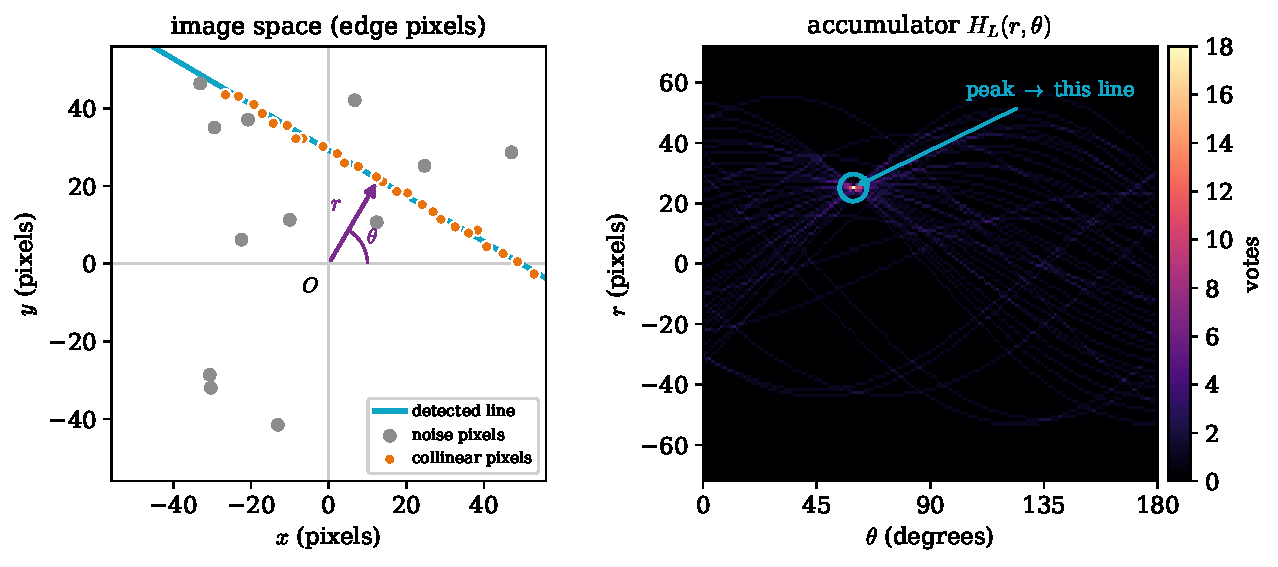
\includegraphics[width=\textwidth]{figures/hough_accumulator.pdf}
  \caption{Image space and parameter space side by side, for a synthetic edge map of
  $26$ collinear pixels (orange) plus $14$ scattered ones (grey). \emph{Left:} the
  edge pixels, with the detected line and its perpendicular parameters $r$ and
  $\theta$ measured from the origin $O$. \emph{Right:} the accumulator
  $H_L(r,\theta)$ drawn as an image. Every edge pixel casts one vote per $\theta$
  column, tracing a sinusoid across the grid; the collinear pixels' sinusoids all
  cross in the same bin, which lights up as the bright peak (circled) at
  $(\theta,r)\approx(60^\circ,25\,\text{px})$, whereas the noise pixels leave only
  faint, uncrossed curves. That peak \emph{is} the line on the left: line detection
  reduces to thresholding this grid for its hottest cells and reading off their
  $(r,\theta)$. Brightness is the number of votes a bin has received.}
  \label{fig:accumulator}
\end{figure}

\paragraph{Using gradients.}
Making every edge pixel sweep over all directions $\theta$ is wasteful, because it
throws away information the edge detector already handed us for free. Finding an
edge means measuring, at each pixel, the direction in which the brightness changes
fastest: the direction of \emph{steepest contrast}, pointing straight across the
boundary from the dark side to the light side. That direction is the image
\emph{gradient}. Now the geometric twist that makes it so useful --- and it is easy
to get backwards. The brightness changes fastest as you step \emph{across} an edge
and barely at all as you walk \emph{along} it, so the gradient points
\emph{perpendicular} to the edge, not along it. The direction of maximum contrast
tells us which way the boundary faces; the edge itself runs at a right angle to
that. But ``perpendicular to the edge'' is precisely the \emph{normal} direction of
the line through the pixel --- the same normal $\hat{\mathbf n}$ whose angle we
named $\theta$ in the Hesse form. The contrast direction therefore hands us
$\theta$ directly, and with it the single line that can pass through that pixel, so
the pixel casts one sharp, well-aimed vote instead of a whole sinusoid of guesses.
To make this concrete, write the gradient of the image brightness as the pair
$\bigl(G_x(x,y),\,G_y(x,y)\bigr)$, the rates of change in the $x$ and $y$
directions (for example the outputs of a Sobel filter). The gradient direction
\begin{equation}
  \theta_G(x,y) = \operatorname{atan2}\!\big(G_y(x,y),\,G_x(x,y)\big)
  \label{eq:gradient-angle}
\end{equation}
\noindent
already fixes the angle $\theta$ of the line through that pixel, so there is no
need to try every $\theta$: we compute the single matching $r$ from
Equation~\eqref{eq:line-rtheta} and update one cell instead of a whole sinusoid.
(The function $\operatorname{atan2}$ is the two-argument arctangent; unlike
$\arctan(G_y/G_x)$ it returns the angle in the correct quadrant and does not
divide by zero when $G_x = 0$.) Finally, a sharp, high-contrast edge is stronger
evidence for a line than a faint one, so instead of adding a flat $+1$ we weight
each vote by the gradient magnitude,
\begin{equation}
  H_L(r,\theta) \;\leftarrow\; H_L(r,\theta)
  + \sqrt{G_x(x,y)^2 + G_y(x,y)^2}\, ,
  \label{eq:hough-vote}
\end{equation}
\noindent
where $\sqrt{G_x^2 + G_y^2}$ is the length of the gradient vector, that is, how
steeply the brightness changes at the pixel. A line in the image then produces a
pronounced maximum in $H_L$, found by the same simple peak detection as before.

\paragraph{Points versus edges.}
The contrast between voting with bare points and voting with oriented edges is
worth keeping in mind, because it recurs in every later method. A bare point is
consistent with infinitely many lines and must vote for all of them (its full
sinusoid), which inflates the chance that unrelated points accidentally agree and
forces a higher peak threshold. An oriented edge, by contrast, carries a
direction, pins down $\theta$ through Equation~\eqref{eq:gradient-angle}, and
votes for essentially one line. The lesson generalizes: the more informative each
piece of local evidence is, the cleaner the peaks and the fewer the false alarms.

\subsection{Detecting Arbitrary Shapes: The Generalized Hough Transform}

Lines are special because they have a tidy two-parameter equation. Most objects
do not: a wrench, a leaf, or a logo is an arbitrary 2D curve with no closed-form
parameterization. Since we cannot write such a shape down as a formula, we instead
\emph{show} it to the algorithm: we supply a \emph{template} --- a single example,
one image of the object or equivalently the 2D curve of its boundary --- that
serves as the known geometric model of exactly the shape we want to find. The
\emph{generalized Hough transform} (GHT) keeps the voting idea but, in place of a
parametric equation, compiles this template into a stored table that records the
shape's geometry explicitly. The detector still asks the same question every edge
can answer with a vote, only now about a shape rather than a line: \emph{if you
are part of this shape, where is its center?}

Everything then splits into two phases built around that template, laid out in
Figure~\ref{fig:ght-template}. \emph{Training} reads the template once and turns it
into the table; \emph{detection} runs the votes on each new test image. We take the
two in turn.

\begin{figure}[ht]
  \centering
  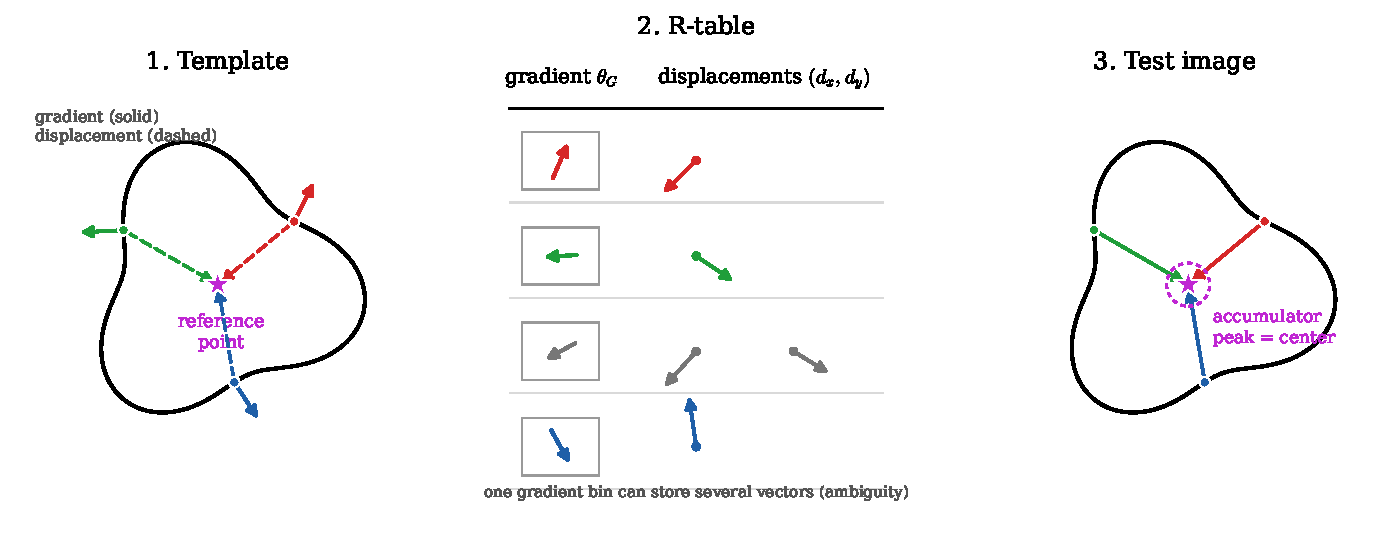
\includegraphics[width=\textwidth]{figures/ght_template.pdf}
  \caption{The generalized Hough transform, from template to detection.
  \emph{(1)~Template:} on the known model shape we fix a reference point (the
  center, magenta star); at each edge we read its gradient direction (solid arrows)
  and record the displacement vector pointing to the center (dashed arrows).
  \emph{(2)~R-table:} those displacements are filed by gradient orientation, so a
  gradient direction indexes straight to the vectors seen at edges facing that way;
  because one orientation can occur at several places on the shape, a single bin may
  hold more than one vector. \emph{(3)~Test image:} each observed edge looks up its
  gradient in the R-table and votes for a center at its position plus the stored
  displacement; edges of a genuine instance all point to the same spot, which wins
  the accumulator peak. Colours track the same edge through all three panels.}
  \label{fig:ght-template}
\end{figure}

\noindent
To set this up we first pick one \emph{reference point} on the template,
typically (but not necessarily) its center of mass. This reference point plays
the role that $(r,\theta)$ played for lines: its position in a test image is what
we are voting for. During training we walk along the template's contour, and for
each edge pixel at position $(x,y)$ we record the \emph{displacement vector}
$(d_x,d_y)$ that points from that edge to the reference point, so that
\begin{equation}
  (x_\text{ref},\,y_\text{ref}) = (x + d_x,\; y + d_y).
  \label{eq:displacement}
\end{equation}
\noindent
The logic at detection time is the mirror image of
Equation~\eqref{eq:displacement}: if an observed edge in the test image is the
same part of the shape, then the center must lie at the edge's own position plus
one of the stored displacements, so the edge votes for those locations. Edges
that genuinely belong to one instance of the shape all point back to the same
spot, which lights up as a peak; unrelated edges scatter their votes harmlessly.

What keeps this efficient is the \emph{R-table}, an indexed list of the
displacement vectors. Just as the gradient orientation accelerated line
detection, it organizes the table here. We quantize the possible gradient
directions into $A$ equal bins (rows). Row $T$ covers gradient orientations near
$\theta \approx 2\pi T/A$ for $T \in \{0,1,\dots,A-1\}$, and it stores every
displacement vector that was observed at an edge with roughly that orientation:
\begin{equation}
  \text{row } T:\quad (d_x^{T,1},d_y^{T,1}),\ (d_x^{T,2},d_y^{T,2}),\ \dots,\
  (d_x^{T,N_T},d_y^{T,N_T}).
  \label{eq:rtable}
\end{equation}
\noindent
Concretely, with $A = 8$ bins each row spans $45^\circ$; an edge whose gradient
points at $100^\circ$ falls in the row centered near $90^\circ$, and we read off
exactly that row's vectors. The superscripts in
Equation~\eqref{eq:rtable} just enumerate the $N_T$ different vectors stored in
row $T$ --- there can be several, which is the point of the next paragraph. At
test time, then, the procedure is: read each edge's gradient orientation, jump to
the matching row, and cast a vote at $(x + d_x, y + d_y)$ for every displacement
$(d_x,d_y)$ in that row.

Why does one row hold several vectors? Because the local gradient is
\emph{ambiguous}: the same gradient direction occurs at several different places
on a shape (think of the two opposite sides of a circle, whose outward normals
are antiparallel, or the many points along a smooth curve that happen to face the
same way). A given orientation is therefore consistent with several possible
centers, so a single observed edge generally increments \emph{several}
accumulator cells, one per displacement in its row. This is not a defect to be
engineered away; it is precisely why voting is needed. Each edge is individually
uncertain about where the center is, but only the true center collects support
from many edges at once. Figure~\ref{fig:ght-rtable} traces this from the model
contour and its displacement vectors through the R-table to the accumulator peak.

Real instances also differ from the stored template in size and orientation. To
handle this, the accumulator gains two more axes and becomes four-dimensional,
$H(x,y,s,\theta)$, where $(x,y)$ is the candidate center, $s$ a scale factor, and
$\theta$ a rotation angle. The two phases are then:
\begin{description}
  \item[Training.] Extract the edge pixels of the template; for each, compute its
    gradient orientation and store the displacement vector to the reference point
    in the corresponding R-table row (Equation~\eqref{eq:rtable}).
  \item[Prediction.] For each scale $s$, multiply the stored displacement vectors
    by $s$; for each rotation $\theta$, rotate the vectors by $\theta$ and shift
    the R-table rows around by the same amount (a circular shift, since rotating
    the shape rotates every edge's gradient by $\theta$); then, for each edge
    pixel in the test image, look up its row, cast a vote from each of its
    displacement vectors, and increment $H(x,y,s,\theta)$. Finally, find the peaks
    in the four-dimensional array.
\end{description}
\noindent
The price of this generality is the four-dimensional search; the reward is a
detector for an \emph{arbitrary} known shape rather than a single parametric
family of lines.

\subsection{Where to Look: Salient Regions}

The generalized Hough transform still assumes we possess an exact template of the
object. That assumption breaks for object \emph{categories}: no two cars, faces,
or motorbikes share one outline, so there is no single contour to store in an
R-table. Before we can let parts vote for an object, we have to decide which image
locations even deserve to be treated as parts. This is the problem of
\emph{saliency}: detecting distinctive regions whose local appearance stands out
from their surroundings, so that the same regions can be found again on a new,
previously unseen instance.

The motivation is partly biological. Saliency is a subjective perceptual quality
that makes certain items capture an observer's attention before others. A standard
computational account mirrors early vision: simple features (color, edge
orientation, luminance, motion) are measured in parallel across the whole field
and at several scales, producing a stack of \emph{feature maps}. Each map is
processed to emphasize locations that differ from their neighbors, the maps are
combined into a single saliency map, and attention --- and, in a living visual
system, the eyes and head --- is drawn to the most salient locations. The idea we
borrow for object models is this notion of ``standing out from the surroundings,''
made mathematically precise and, importantly, invariant to scale and rotation so
that detections repeat across instances.

The Kadir/Brady detector makes ``standing out'' concrete by equating saliency with
\emph{rareness}, measured through Shannon entropy. The reason rareness needs a
careful definition is that it is easy to get trivially wrong: if our description
of a patch is so specific that every location looks unique, then everything is
equally rare; if it is so generic that everything looks alike, nothing is rare.
Entropy of the local intensity distribution sits between these extremes and
measures the \emph{complexity} of a patch. For a window of pixels, let $p(k)$ be
the fraction of pixels whose grey value equals $k$, for $k = 0,\dots,255$; this
is just the normalized local histogram. The entropy is
\begin{equation}
  H = -\sum_{k=0}^{255} p(k)\log_2 p(k),
  \qquad \text{with the convention } 0\log_2 0 = 0 .
  \label{eq:entropy}
\end{equation}
\noindent
Each term $-p(k)\log_2 p(k)$ is the contribution of grey level $k$; summing them
gives the average number of \emph{bits} needed to encode a pixel drawn from the
window, which is also a measure of how uncertain we are about that pixel's value.
A couple of concrete windows fix the intuition. If every pixel has the same grey
value, one $p(k)$ equals $1$ and the rest are $0$, so $H = 0$: a flat, predictable
patch carries no information. If the window contains two grey values in equal
numbers, two terms equal $-\tfrac12\log_2\tfrac12 = \tfrac12$ and $H = 1$ bit. If
all $256$ levels are equally likely, $p(k) = 1/256$ for each and $H = \log_2 256 =
8$ bits, the maximum. So a \emph{flatter} local histogram means \emph{higher}
entropy, and a textured, unpredictable patch is rare in this spatial sense, while
a smooth or constant patch is not.

High spatial entropy alone is still not enough, because pure noise also has a flat
histogram yet is not distinctive: its statistics barely change as the analysis
window grows, so it looks the same at every scale. We therefore add a second
requirement, \emph{self-dissimilarity in scale}: a salient region should look
different at its own scale than at nearby scales. To express this we analyze each
location over a range of window sizes (a Gaussian scale space, or an image pyramid
that subsamples in logarithmic steps), and treat entropy as a function of the
scale $s$. Writing $p(I,s,x)$ for the probability density of intensity value $I$
inside a window of scale $s$ centered at position $x$, the scale-dependent entropy
and the scales at which it peaks are
\begin{equation}
  H_D(s,x) = -\!\int p(I,s,x)\,\log_2 p(I,s,x)\,\mathrm{d}I,
  \qquad
  s_p = \Big\{\, s : \tfrac{\partial H_D}{\partial s}=0,\
  \tfrac{\partial^2 H_D}{\partial s^2}<0 \,\Big\}.
  \label{eq:scale-entropy}
\end{equation}
\noindent
Equation~\eqref{eq:scale-entropy} is just Equation~\eqref{eq:entropy} written for
a continuous intensity $I$ and made a function of scale; the condition on $s_p$ is
the textbook test for a local maximum (first derivative zero, second derivative
negative), so $s_p$ collects the scales where the entropy curve has a \emph{peak}.
Each such peak is then reweighted by how strongly the intensity distribution
itself changes with scale,
\begin{equation}
  W_D(s,x) = s\!\int \Big| \tfrac{\partial}{\partial s} p(I,s,x) \Big|\,\mathrm{d}I,
  \qquad
  y(s_p,x) = H_D(s_p,x)\,W_D(s_p,x).
  \label{eq:saliency-weight}
\end{equation}
\noindent
The weight $W_D$ is large when the distribution looks markedly different at scale
$s$ than at neighboring scales (the $|\partial p/\partial s|$ term), with the
leading $s$ making the measure comparable across scales; the final saliency
$y(s_p,x)$ is the product, so a location scores highly only when it is both
complex (high $H_D$) and tied to a distinctive scale (high $W_D$). This is exactly
what suppresses featureless noise, whose entropy is high but flat across scale.
Figure~\ref{fig:saliency-scale} shows the entropy-versus-scale curve with its
peak, alongside the flat-versus-peaked histogram intuition.

In practice the algorithm visits each pixel, computes the local entropy
(Equation~\eqref{eq:entropy}) over a range of scales, keeps the scales where the
entropy peaks (there may be none), and weights those entropies by the inter-scale
change of the distribution. Run on a dataset such as side views of motorbikes,
and averaged over many images, the detected salient points cluster on repeatable,
characteristic object parts --- wheels, the engine block, the seat --- which is
precisely the raw material the next models need.

This is the \emph{classical} stance on saliency: hand-crafted features grounded in
information theory, computed without learning, and largely task-independent (data
enter only at evaluation time). The \emph{modern} alternative is to learn saliency
from data with deep networks, building on the multilayer perceptrons and
convolutional networks of Section~\ref{sec:neural-networks}; a convolutional
network trades hand-designed rareness for features learned from many labeled
examples, at the cost of needing a great deal of such data. We stay with the
classical view here because it makes explicit \emph{why} a location is worth voting
from.

\subsection{What to Record: Local Features and Shape Descriptors}

Saliency tells us \emph{where} to look; a descriptor decides \emph{what} to record
there, encoding the neighborhood as a vector so that the same part can be matched
again on a new image. What makes one descriptor better than another is best
understood as a balancing act among four competing demands, summarized in
Table~\ref{tab:feature-criteria}.

\begin{table}[ht]
  \centering
  \begin{tabular}{@{}p{3.0cm}p{10.5cm}@{}}
    \toprule
    Property & What it means \\
    \midrule
    Invariance & Stays stable under nuisance changes: translation, rotation,
      scale, and illumination. \\
    Discriminability & Separates similar classes reliably; different parts get
      different descriptors. \\
    Compactness & Stores enough information in a short vector to keep matching
      and storage cheap. \\
    Computational cost & Remains feasible to extract and compare on large
      datasets. \\
    \bottomrule
  \end{tabular}
  \caption{The four criteria for a good local feature. Invariance and
  discriminability pull in opposite directions, and compactness and cost bound
  how far either can be pushed.}
  \label{tab:feature-criteria}
\end{table}

\noindent
These demands genuinely conflict. Pushing invariance to the limit deliberately
discards information --- if a descriptor is built to ignore rotation, it can no
longer tell two parts apart that differ only by rotation --- which eats into
discriminability. And richer, more discriminative descriptors are longer and
costlier to compute and compare. Every concrete descriptor is one particular
compromise among the four.

The \emph{histogram of oriented gradients} (HOG) is the canonical compromise on
the shape-and-appearance side, and it is worth seeing how it is built because it
reuses the gradients from Equation~\eqref{eq:hough-vote}. The region is divided
into a grid of small \emph{cells}; within each cell the gradient orientations of
the pixels are collected into a histogram (for example over nine orientation
bins), each pixel contributing in proportion to its gradient magnitude. Cells are
then grouped into overlapping \emph{blocks}, and the histograms in a block are
normalized together before being concatenated, over all blocks, into one long
feature vector. Figure~\ref{fig:hog} shows the whole construction on a simple
shape. Two design choices give HOG its character. Summarizing gradient
\emph{orientations} rather than raw intensities, together with the block
normalization, makes it robust to moderate lighting changes and small
deformations. But because the descriptor is laid out as a fixed grid of oriented
histograms, rotating the patch permutes the bins and changes the vector: standard
HOG is \emph{not} rotation invariant. In return it turns the diffuse evidence of
many edges into a single classifier-ready vector, which is why it remains a
standard baseline against which learned features are measured.

\begin{figure}[ht]
  \centering
  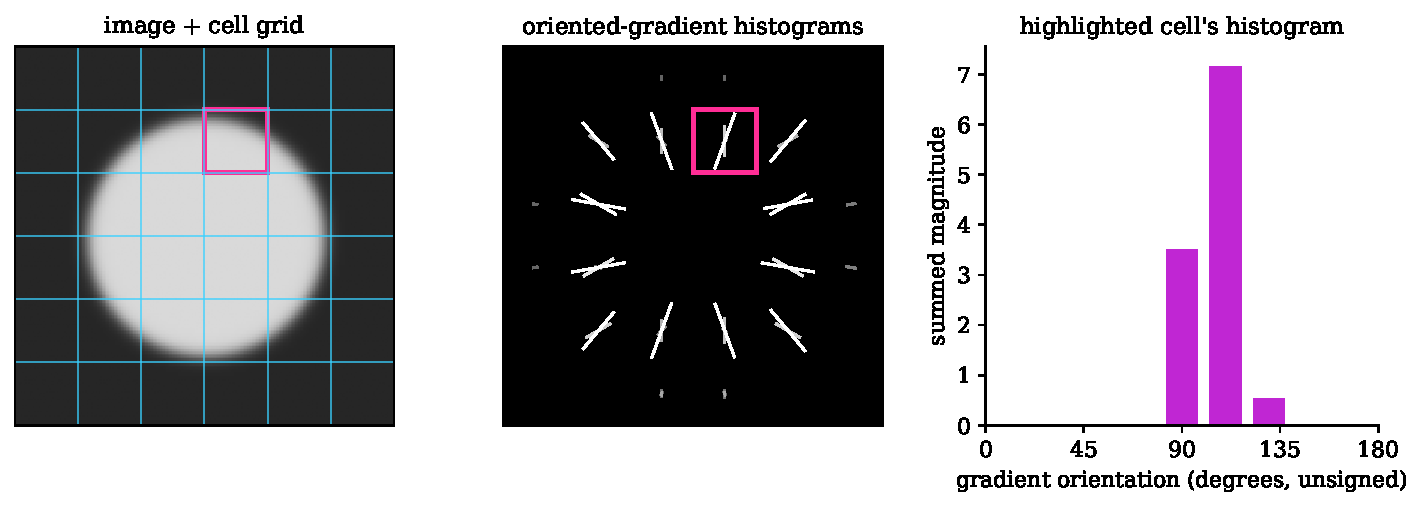
\includegraphics[width=\textwidth]{figures/hog_descriptor.pdf}
  \caption{Building a HOG descriptor, computed on a synthetic disk.
  \emph{Left:} the region is divided into a grid of cells (one highlighted in
  magenta). \emph{Middle:} each cell is replaced by a small star of strokes, one
  per orientation bin, whose length is the total gradient magnitude falling in that
  orientation; since gradients run perpendicular to edges, the strokes point
  radially around the disk's rim, while flat interior and exterior cells stay
  empty. \emph{Right:} the highlighted cell's nine-bin histogram of gradient
  orientation, each pixel weighted by its gradient magnitude, with a clear peak at
  the orientation of the local edge. Stacking every cell's (block-normalized)
  histogram into one vector yields the descriptor.}
  \label{fig:hog}
\end{figure}

Two further descriptor families round out the classical toolkit and contrast
usefully with HOG. \emph{Fourier descriptors} encode a closed contour by the
Fourier coefficients of its boundary curve; translation, rotation, and scaling of
the shape act on those coefficients in simple, separable ways (a shift of the
constant term, a phase change, an overall magnitude scaling), so after
normalization the coefficients become invariant shape descriptors. \emph{Hu
moments} combine image moments into a handful of quantities that are likewise
invariant to translation, scale, and rotation. For detecting the salient
\emph{points} in the first place, the standard keypoint operators (Harris,
Förstner, SIFT) provide the geometric counterpart to the information-theoretic
salient regions of the previous subsection. The common thread across all of them
is the same: a descriptor converts a neighborhood into a compact vector, and
closeness between two such vectors is taken to mean that the two patches show the
same thing.

\subsection{Putting It Together: The Implicit Shape Model}

The implicit shape model (ISM) is where the three threads of this section ---
voting, saliency, and description --- finally meet. Its goal is object
\emph{categorization} in real scenes: given training images of a category, learn a
model from the local appearance of its parts; given a new image, both label and
segment the instances. The one-sentence summary is that ISM is a generalized
Hough transform whose fixed geometric R-table has been replaced by a \emph{learned
appearance codebook}. Where the GHT indexed displacement vectors by an edge's
gradient orientation, ISM indexes them by a patch's appearance; the voting
machinery is otherwise the same.

The \textbf{training phase} builds that codebook. Salient points are extracted
from the training images (using the salient-region or keypoint detectors above),
and each one defines a \emph{patch} at its characteristic scale. The patches are
described by their local appearance and then grouped so that visually similar
patches become a single \emph{codebook} entry --- a prototype part such as ``front
wheel'' or ``headlight.'' The grouping is done by iterative merging: every patch
starts as its own cluster, and at each step the two most similar clusters $C_1$
and $C_2$ are merged, provided their average pairwise similarity stays above a
threshold $t$. Similarity between two patches $p$ and $q$ is the normalized
greyscale correlation, and the similarity of two clusters averages it over all
their members:
\begin{equation}
  \mathrm{NGC}(p,q) = \frac{\sum_i (p_i-\bar p)(q_i-\bar q)}
  {\sqrt{\sum_i (p_i-\bar p)^2 \;\sum_i (q_i-\bar q)^2}},
  \qquad
  \mathrm{sim}(C_1,C_2) = \!\!\sum_{p\in C_1,\,q\in C_2}\!\!
  \frac{\mathrm{NGC}(p,q)}{|C_1|\,|C_2|}.
  \label{eq:ngc}
\end{equation}
\noindent
In $\mathrm{NGC}(p,q)$, the index $i$ runs over the pixels of the patch, $p_i$ and
$q_i$ are their grey values, and $\bar p,\bar q$ are the patch means; subtracting
the means removes brightness offsets and the denominator removes contrast
scaling, so $\mathrm{NGC}$ is a correlation coefficient between $-1$ and $1$ that
equals $1$ for patches identical up to brightness and contrast and near $0$ for
unrelated ones. The cluster similarity $\mathrm{sim}(C_1,C_2)$ is then just the
average $\mathrm{NGC}$ over all cross-pairs, with $|C_i|$ the number of patches in
cluster $C_i$. Stopping the merges at the threshold $t$ keeps clusters compact and
groups only genuinely similar patches. Finally, for each codebook entry we record,
across all the training images, the offset vectors from every matching patch to
the object center --- the appearance analogue of the R-table's displacement
vectors, specifying where on the object each prototype part tends to appear.

The \textbf{prediction phase} runs the voting. Salient patches are extracted from
the test image and matched against the codebook; an entry is \emph{activated}
whenever its $\mathrm{NGC}$ similarity to a patch exceeds the threshold $t$. Each
activated entry then casts generalized Hough votes for the object center, placing
a vote at the patch position plus each of that entry's stored offsets --- exactly
the GHT step, but driven by appearance rather than edge orientation. Unlike the
discrete accumulator of the classical GHT, ISM votes in a \emph{continuous} space,
and the densest cluster of votes is located with mean-shift mode estimation
(equivalently, a non-parametric density estimate); that mode is the hypothesized
object center. A final \emph{back-projection} step reverses the voting: the
patches that supported the winning center are projected back into the image, which
both localizes the object within a surrounding region and, through a probabilistic
formulation, yields a pixel-level \emph{segmentation} rather than a mere bounding
box. Figure~\ref{fig:ism-pipeline} lays out the whole pipeline, training above and
prediction below.

Because ISM grows directly out of the generalized Hough transform, it helps to see
the two side by side; Table~\ref{tab:ght-vs-ism} lines up what changes and what
stays the same.

\begin{table}[ht]
  \centering
  \begin{tabular}{@{}p{3.2cm}p{5.0cm}p{5.0cm}@{}}
    \toprule
    Aspect & Generalized Hough transform & Implicit shape model \\
    \midrule
    Model of a part & Fixed geometric R-table & Learned appearance codebook \\
    Local evidence & Edge + gradient orientation & Salient patch + appearance \\
    Indexing & Gradient-orientation row & Codebook match above threshold $t$ \\
    Voting space & Discrete accumulator & Continuous (mean-shift modes) \\
    Output & Center / pose of one known shape & Category detection \emph{and}
      segmentation \\
    \bottomrule
  \end{tabular}
  \caption{From a single known shape to an object category: ISM keeps the voting
  machinery of the generalized Hough transform but learns the parts and their
  spatial distribution from data.}
  \label{tab:ght-vs-ism}
\end{table}

\noindent
Two further models slot naturally into the same picture. \emph{Hough forests}
replace the codebook-and-matching step with a random forest that maps each patch
directly to a distribution of votes, learning the appearance grouping and the
offsets together in one trained predictor. \emph{Deformable part models} (DPM)
take a complementary route: an object is a coarse root HOG template plus a few
higher-resolution part templates attached to it by spring-like deformation costs,
the whole thing scored with a latent-variable classifier. Both keep the central
bargain of this section --- local parts proposing global configurations --- while
changing how the parts are represented and how their votes are combined. The
implicit shape model itself is due to Leibe, Leonardis, and Schiele (ECCV'04
workshop; IJCV 2008).

It is worth ending where we began. Every model in this section is one instance of
the same mechanism, differing only in what counts as local evidence and how much
flexibility the global hypothesis is allowed; Table~\ref{tab:voting-recap} lines
them up along that single axis.

\begin{table}[ht]
  \centering
  \begin{tabular}{@{}p{3.6cm}p{4.6cm}p{5.4cm}@{}}
    \toprule
    Model & What casts a vote & What it votes for \\
    \midrule
    Hough line detector & An oriented edge pixel & The line $(r,\theta)$ it lies
      on \\
    Generalized Hough transform & An edge, indexed by gradient orientation & The
      reference center of a known shape, in $(x,y,s,\theta)$ \\
    Implicit shape model & A patch matched to a codebook entry & The object
      center, in a continuous space, then a segmentation \\
    \bottomrule
  \end{tabular}
  \caption{The through-line of the section. As the local evidence grows richer ---
  from edge to oriented edge to learned appearance patch --- the same voting
  scheme stretches from a single line to an arbitrary shape to a whole object
  category.}
  \label{tab:voting-recap}
\end{table}
